\documentclass{article}
\usepackage{amsmath}
\usepackage{amsfonts}
\usepackage{float}
\usepackage{pgfplots}
\pgfplotsset{compat=1.18}

\begin{document}

\section*{Varianza del estimador de MCO con  heterocedasticidad}

Consideremos el modelo de regresión lineal:
\[
y = X \beta + u
\]
donde:
- \( y \) es el vector de \( n \) observaciones de la variable dependiente,
- \( X \) es la matriz de diseño de \( n \times k \) que incluye las variables explicativas,
- \( \beta \) es el vector de \( k \) parámetros a estimar,
- \( u \) es el vector de errores aleatorios de tamaño \( n \).

En este caso, suponemos que existe heterocedasticidad en los errores, lo que significa que la matriz de varianzas-covarianzas de los errores \( u \) no es esférica. En lugar de asumir homocedasticidad (\( \mathbb{E}(uu') = \sigma^2 I \)), asumimos que:
\[
\mathbb{E}(uu') = \Omega
\]
donde \( \Omega \) es una matriz de varianzas-covarianzas \( n \times n \), que refleja que las varianzas pueden cambiar entre las observaciones.

\[
\boldsymbol{\Omega} =
\begin{bmatrix}
\sigma_1^2 & 0 & \cdots & 0 \\
0 & \sigma_2^2 & \cdots & 0 \\
\vdots & \vdots & \ddots & \vdots \\
0 & 0 & \cdots & \sigma_n^2
\end{bmatrix}
\]

El estimador de mínimos cuadrados ordinarios (MCO) para \( \beta \) se define como:
\[
\hat{\beta}_{\text{MCO}} = (X'X)^{-1} X'y
\]

Sustituyendo \( y = X \beta + u \) en esta expresión, obtenemos:
\[
\hat{\beta}_{\text{MCO}} = (X'X)^{-1} X'(X \beta + u)
\]

Al desarrollar, esto se convierte en:
\[
\hat{\beta}_{\text{MCO}} = \beta + (X'X)^{-1} X'u
\]


Queremos encontrar la varianza de \( \hat{\beta}_{\text{MCO}} \), es decir, \( \text{Var}(\hat{\beta}_{\text{MCO}}) \).

Dado que \( \hat{\beta}_{\text{MCO}} = \beta + (X'X)^{-1} X'u \), podemos escribir:
\[
\text{Var}(\hat{\beta}_{\text{MCO}}) = \text{Var}((X'X)^{-1} X'u)
\]

Utilizando la propiedad de que \( \text{Var}(A u) = A \, \text{Var}(u) \, A' \), tenemos:
\[
\text{Var}(\hat{\beta}_{\text{MCO}}) = (X'X)^{-1} X' \, \text{Var}(u) \, X (X'X)^{-1}
\]


Como hemos supuesto que \( \text{Var}(u) = \Omega \), sustituimos esto en la expresión anterior:
\[
\text{Var}(\hat{\beta}_{\text{MCO}}) = (X'X)^{-1} X' \Omega X (X'X)^{-1}
\]



Si \( \Omega = \sigma^2 I \) (homocedasticidad), entonces la expresión se reduce a:
\[
\text{Var}(\hat{\beta}_{\text{MCO}}) = \sigma^2 (X'X)^{-1}
\]


\section*{Perturbaciones esféricas y no esféricas}

\begin{figure}[H]
  \centering
  \begin{minipage}{0.5\textwidth}
    \centering
    
\includegraphics[width=\linewidth]{image.png}
   % \caption*{Esférica}
  \end{minipage}\hfill
  \begin{minipage}{0.5\textwidth}
    \centering
    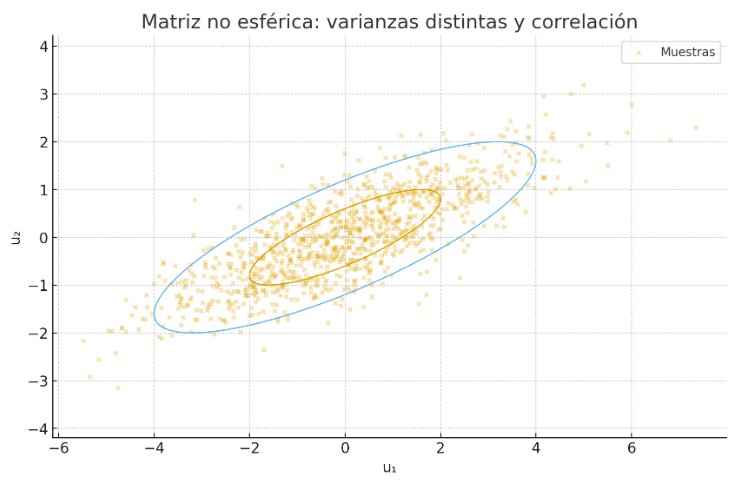
\includegraphics[width=\linewidth]{no_esf.png}
   % \caption*{No esférica}
  \end{minipage}
  \caption{Comparación de perturbaciones esféricas y no esféricas.}
\end{figure}

\textbf{Curvas de isoprobabilidad:}  
Las líneas del gráfico representan \textit{curvas de isoprobabilidad} (o de igual densidad) de la distribución conjunta de los errores. Cada curva une los puntos $(u_1,u_2)$ que tienen la misma probabilidad de ocurrencia bajo la distribución de los errores.

En el caso de errores normales con matriz de varianzas–covarianzas $\Omega$, la densidad conjunta se expresa como
\[
f(u) = \frac{1}{2\pi |\Omega|^{1/2}} 
\exp\!\left(-\tfrac{1}{2}u'\Omega^{-1}u\right).
\]
De esta forma, las curvas de nivel que satisfacen $u'\Omega^{-1}u = c$ describen las regiones de igual probabilidad.

La \textbf{mayor probabilidad} se encuentra en el centro de la distribución, en el punto $(0,0)$, donde la densidad es máxima.  
Es decir, las curvas más cercanas al centro representan valores más probables, mientras que las curvas más externas corresponden a valores menos probables.


\end{document}
